\section{Results and Discussion} \label{sec:results}

../../tex/lib/importpath.tex

\begin{figure*}%
%-------------------------------------------------------------------------------
  \begin{subfigure}[b]{0.33\linewidth}
    \centering
    % pass an arbitrary filename, potentially with unsafe characters
    % adapted from https://tex.stackexchange.com/a/36178
    \catcode`\%=12
    \providecommand\filename{}
    \renewcommand\filename{\detokenize{submodules/hereditary-stratigraph-concept-binder/binder/phylogenetic-inference/teeplots/a=true_phylogeny+source=a%reconstructed_phylogenies~source%nk_lexicaseselection_seed110_pop165_mut.01_snapshot_500.csv.gz+viz=truncate-phylo+ext=}}
    \catcode`\%=14
    \includegraphics[width=\linewidth]{\importpath\filename}
    \caption{Ground truth phylogeny.}
    \label{fig:reconstruction-example-true-phylogeny}
  \end{subfigure}%
%-------------------------------------------------------------------------------
  \begin{subfigure}[b]{0.33\linewidth}
    \centering
    % pass an arbitrary filename, potentially with unsafe characters
    % adapted from https://tex.stackexchange.com/a/36178
    \catcode`\%=12
    \providecommand\filename{}
    \renewcommand\filename{\detokenize{submodules/hereditary-stratigraph-concept-binder/binder/phylogenetic-inference/teeplots/source=a%reconstructed_phylogenies~source%nk_lexicaseselection_seed110_pop165_mut.01_snapshot_500.csv.gz+treatment=differentia%1~policy%TaperedDepthProportionalResolution~target%64+viz=truncate-phylo-bounds+ext=}}
    \catcode`\%=14
    \includegraphics[width=\linewidth]{\importpath\filename}
    \caption{1-bit Fingerprint Differentia, Tapered Depth-Proportional Resolution Stratum Retention Predicate, 64 bit target column footprint.}
    \label{fig:reconstruction-example-d1-rp-t64}
  \end{subfigure}%
%-------------------------------------------------------------------------------
  \begin{subfigure}[b]{0.33\linewidth}
    \centering
    % pass an arbitrary filename, potentially with unsafe characters
    % adapted from https://tex.stackexchange.com/a/36178
    \catcode`\%=12
    \providecommand\filename{}
    \renewcommand\filename{\detokenize{submodules/hereditary-stratigraph-concept-binder/binder/phylogenetic-inference/teeplots/source=a%reconstructed_phylogenies~source%nk_lexicaseselection_seed110_pop165_mut.01_snapshot_500.csv.gz+treatment=differentia%1~policy%RecencyProportionalResolution~target%64+viz=truncate-phylo-bounds+ext=}}
    \catcode`\%=14
    \includegraphics[width=\textwidth]{\importpath\filename}
    \caption{1-bit Fingerprint Differentia, MRCA-Recency-Proportional Resolution Stratum Retention Predicate, 64 bit target column footprint.}
    \label{fig:reconstruction-example-d1-tdp-t64}
  \end{subfigure}
%-------------------------------------------------------------------------------
  \caption{
    Example phylogeny reconstructions of ground-truth lexicase selection phylogeny from inference on extant hereditary stratigraphic columns.
    Shaded error bars on reconstructions indicate 95\% confidence intervals for the true generation of tree nodes.
    Arbitrary color is added to enhance distinguishability.
  }
  \label{fig:reconstruction-example}
\end{figure*}


In this section, we analyze the quality of reconstructions of known phylogenetic trees using hereditary stratigraphy.
Figure \ref{fig:reconstruction-example} compares an example reconstruction from columns using tapered depth-proportional stratum retention, an example reconstruction using recency-proportional stratum retention,  and the underlying ground truth phylogeny.
Interactive in-browser visualizations comparing all reconstructed phylogenies to their corresponding ground truth are available at \url{https://hopth.ru/bi}. %TODO: replace this with anonymous link

\subsection{Reconstruction Accuracy}

Measuring tree similarity is a challenging problem, with many conflicting approaches that all provide different information \citep{smith2020treedist}.
Ideally, we would use a metric of reconstruction accuracy that 1) is commonly used so that there exists sufficient context to understand what constitutes a good value, 2) behaves consistently across different types of trees, and 3) behaves reasonably for the types of trees common in artificial life data.
Unfortunately, these objectives are somewhat in conflict.
The primary source of this problem is multifurcations, nodes from which more than two lineages branch at once.
In reconstructed phylogenies in biology, multifurcations are generally assumed to be the result of insufficient information.
It is thought that the real phylogeny had multiple bifurcations that occurred so close together that the reconstruction algorithm is unable to separate them.
In artificial life phylogenies, however, we have the opposite problem.
When we perfectly track a phylogeny, it is common for us to know that a multifurcation did in fact occur.
However, it is challenging for our reconstructions to properly identify multifurcations, because it requires perfectly lining up multiple divergence times.
Many of the most popular tree distance metrics interpret the difference between a multifurcation and a set of bifurcations as a dramatic change in topology.
For some use cases, this change in topology may indeed be meaningful, although research on the extent of this problem is limited.
Nevertheless, we suspect that for the majority of use cases, the tiny branch lengths between the internal nodes will make this source of error relatively minor.

To overcome this obstacle, we have measured our reconstruction accuracy using multiple metrics.
We will primarily focus on Mutual Clustering Information (as implemented in the R TreeDist package) \citep{smith2020treedist}, which is a direct measure of the quantity of information in the ground truth phylogeny that was successfully captured in the reconstruction.
It is relatively unaffected by the failure to perfectly reproduce multifurcations.
For the purposes of easy comparison to the literature, we also measured the Clustering Information Distance \citep{smith2020treedist}.

\begin{figure}
    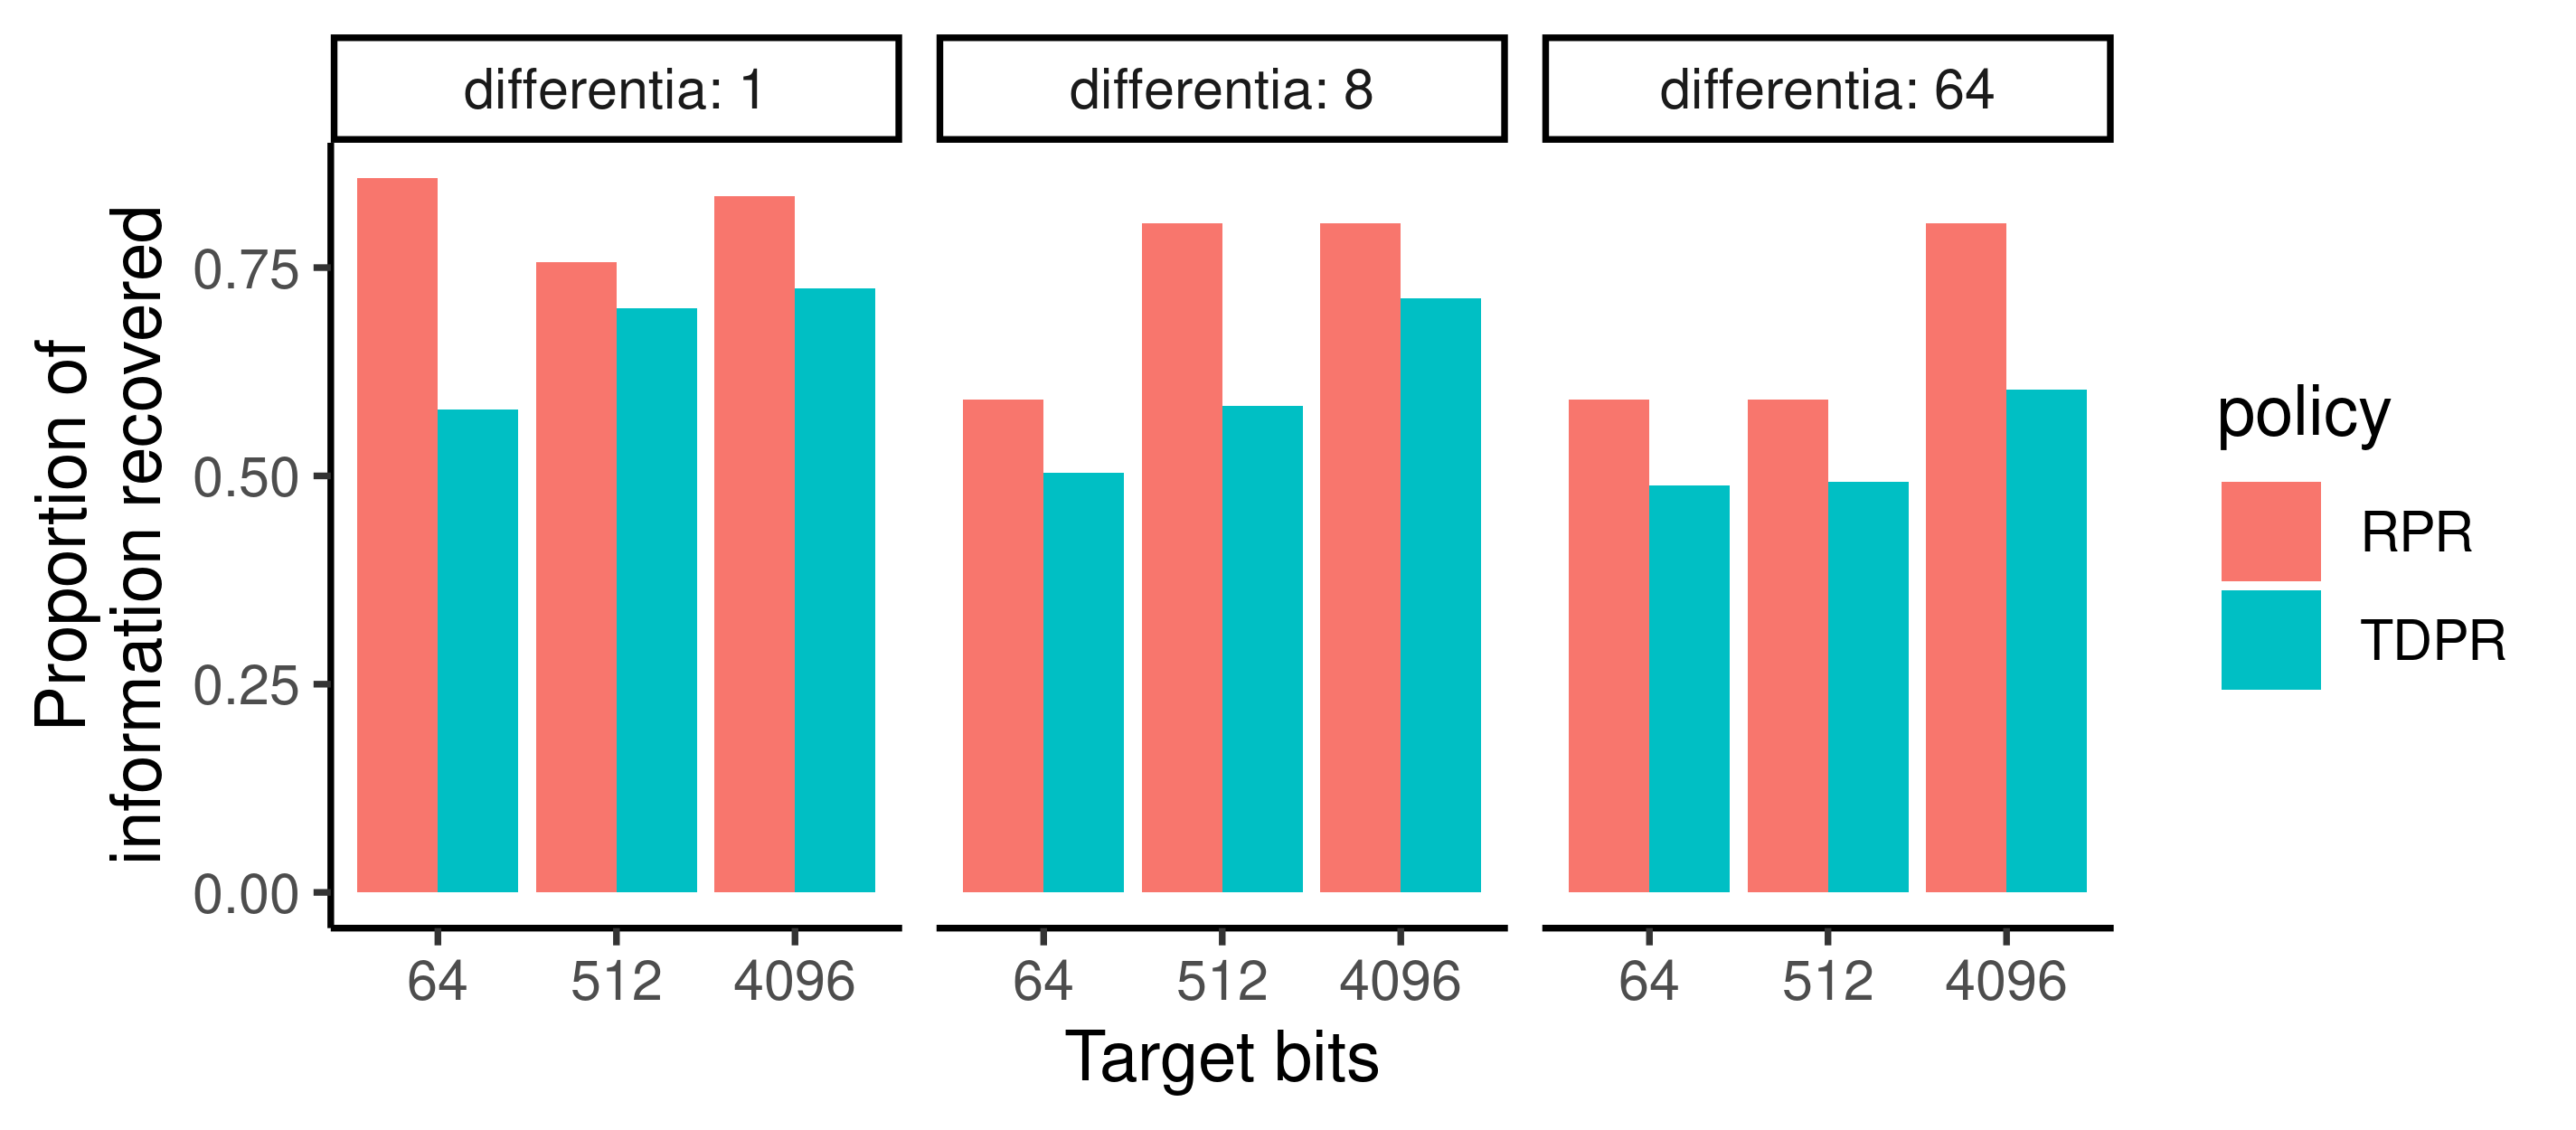
\includegraphics[width=\columnwidth]{img/info_plot}
    \caption{
    Proportion of information present in the ground-truth ftness sharing phylogeny that was captureed by our reconstruction, across various retention policies.
    High is better (1 is perfect).
    RPR is recency-proportional resolution policy and TDPR is tapered depth-proportional resolution policy.
    } \label{fig:info_plot}
\end{figure}

Across ground truth phylogenies, we were able to reconstruct the phylogenetic topology with between 47.75\% and 85.70\% of the information contained in the original tree using a 64-bit column memory footprint, between 47.75\% and 80.36\% using a 512-bit column memory footprint, and between 51.13\% and 83.53\% using a 4096-bit column memory footprint.
While the Clustering Information Distance reached its maximum possible score (1.0) for the heavily-multifurcated EcoEA phylogeny, it agreed with the Mutual Clustering Information score for less multifurcated phylogenies, such as fitness sharing.
Using the Recency Proportional Resolution retention policy and a 4096-bit column memory footprint, we were able to reconstruct a fitness sharing phylogeny with a Clustering Information Distance of only 0.2923471 from the ground truth.
For context, that result is comparable to the distance between phylogenies reconstructed from two closely-related proteins in H3N2 flu (0.25) \citep{jones2021parallel}.
To build further intution, we strongly encourage readers to refer to our interactive web reconstruction.
Figure \ref{fig:info_plot} summarizes error reconstructing the fitness sharing selection phylogeny in terms of the mutual clustering information metric \citep{smith2022robust}.
The phylogenies reconstructed from the EcoEA conddition performed comparably, with lexicase and random selection faring somewhat worse \citep{moreno2022hstratconceptsupplement}. %TODO cite supplement
In the case of random selection, we suspect that this reduced performance is the result of having many nodes that originated very close together at the end of the experiment.
As expected, we did observe overall more accurate reconstructions from columns that were allowed to occupy larger memory footprints.

\subsection{Differentia Size}

Among the surveyed ground truth phylogenies and target column footprints, we consistently found that smaller differentia were able to yield more or as accurate phylogenetic reconstructions.
The stronger performance of narrow differentia was particularly apparent in low-memory-footprint scenarios where overall phylogenetic inference power was weaker.
Overall, single-bit differentia outperformed 64-bit differentia under 20 condtions, and were indistinguishable under 7 conditions, and were worse under 3 conditions.
Full results are available in Supplementary Section \ref{sec:differentia-size-full}.
Although narrower differentia have less distinguishing power on their own, their smaller size allows more to be packed into the memory footprint to cover more generations, which seems to help reconstruction power.
We must note that narrower differentia can pack more thoroughly into the footprint caps we imposed on column size, so their extant columns tended to have slightly more overall bits.
However, this was a small enough imbalance (in most cases $<10\%$) that we believe it is unlikely to fully account for the stronger performance of narrow-differentia configurations.

\subsection{Retention Policy}

Across the surveyed ground truth phylogenies and target column memory footprints, we found that the recency-proportional resolution stratum retention policy generally yielded better phylogenetic reconstructions.
Phylogenetic reconstruction quality was better in 28 conditions, equivalent in 14 conditions, and worse in 3 conditions.
Again, this effect was most apparent in the small-stratum-count scenarios where overal inference power was weaker.
Full results are available in Supplementary Section \ref{sec:retention-policy-full}.
The stronger performance of recency-proportional resolution is likely due to the denser retention of recent strata under the recency-proportional metric, which help to resolve the more numerous (and therefore typically more tightly spaced) phylogenetic events in the near past \citep{zhaxybayeva2004cladogenesis}.
Recency-proportional resolution tended to be able to fit fewer strata within the prescribed memory footprints (except in cases where it could not fit within the footprint) so its stronger performance cannot be attributed to more retained bits in the end-state extant columns.
